\chapter{总体设计}
\label{cha:design}

\section{系统结构}

如 \ref{sec:Larvel} 中所述, UNIT3D按照标准的Laravel项目组织文件。根据开发需要, 笔者需要增删修改的主要有`/app/Http/Controllers/, /app/Http/Controllers/API/, /app/Models/, /database/migrations/, /resources/views/, /resources/lang/', 分别对应投票、增添新字段所应修改的控制器部分, 数据结构模型部分, 数据库表迁移部分, 资源的视图部分, 以及本地化的语言词汇对照部分。

\begin{figure}[!ht]
	\centering
    \begin{subfigure}{0.3\textwidth}
		\centering
		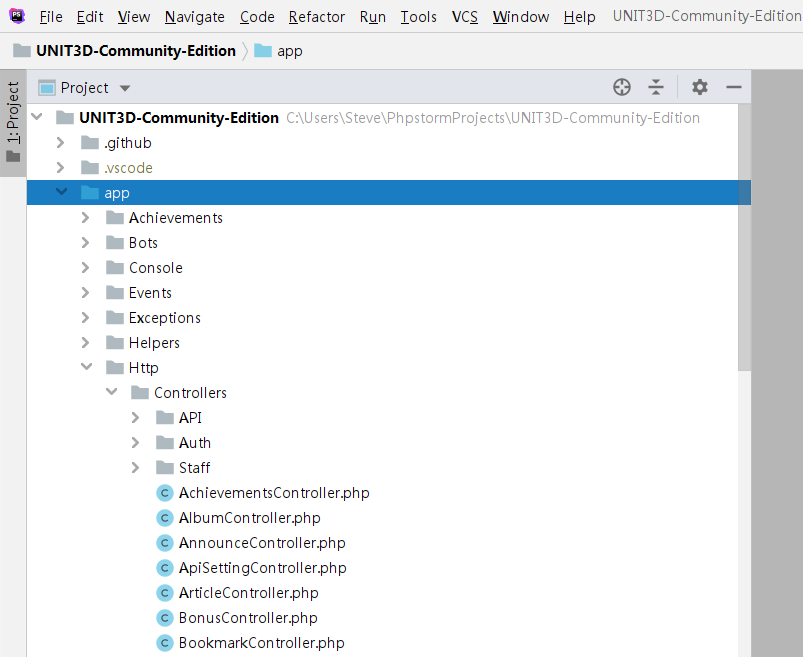
\includegraphics[width=\textwidth]{support-files/3.1-phpstorm-folder-structure-1.png}
		\caption{ }
		\label{fig:torrent_in_bencode}
	\end{subfigure} 
	\makebox[0.05\textwidth]{}
    \begin{subfigure}{0.3\textwidth}
		\centering
		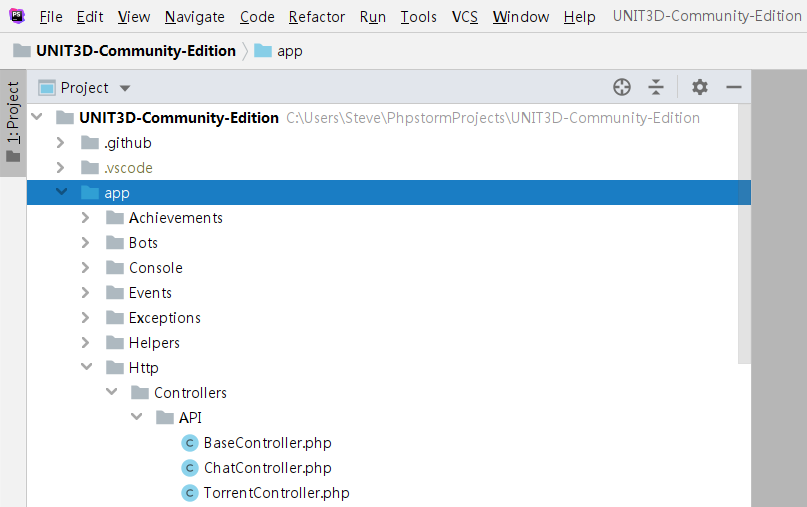
\includegraphics[width=\textwidth]{support-files/3.1-phpstorm-folder-structure-2.png}
		\caption{ }
		\label{fig:torrent_in_bencode}
	\end{subfigure} \\
	% \makebox[0.05\textwidth]{}
    \begin{subfigure}{0.3\textwidth}
		\centering
		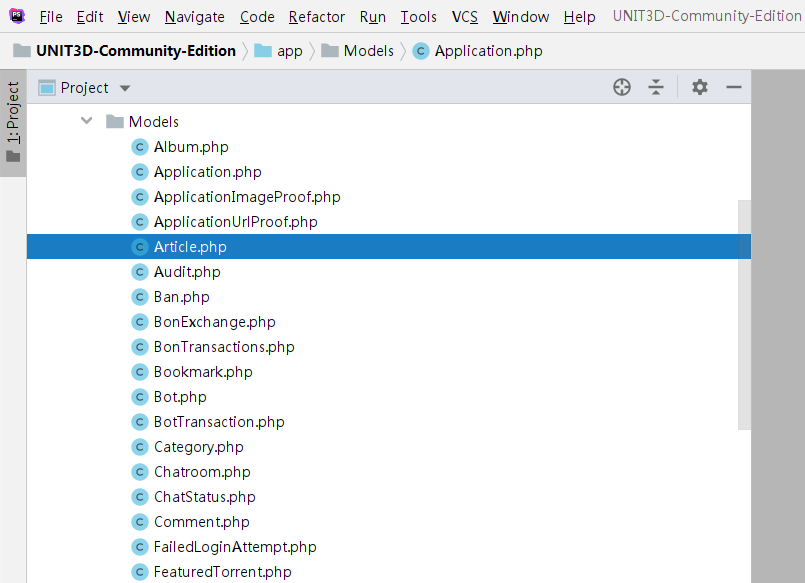
\includegraphics[width=\textwidth]{support-files/3.1-phpstorm-folder-structure-3.png}
		\caption{ }
		\label{fig:torrent_in_bencode}
	\end{subfigure} 
	\makebox[0.05\textwidth]{}
    \begin{subfigure}{0.3\textwidth}
		\centering
		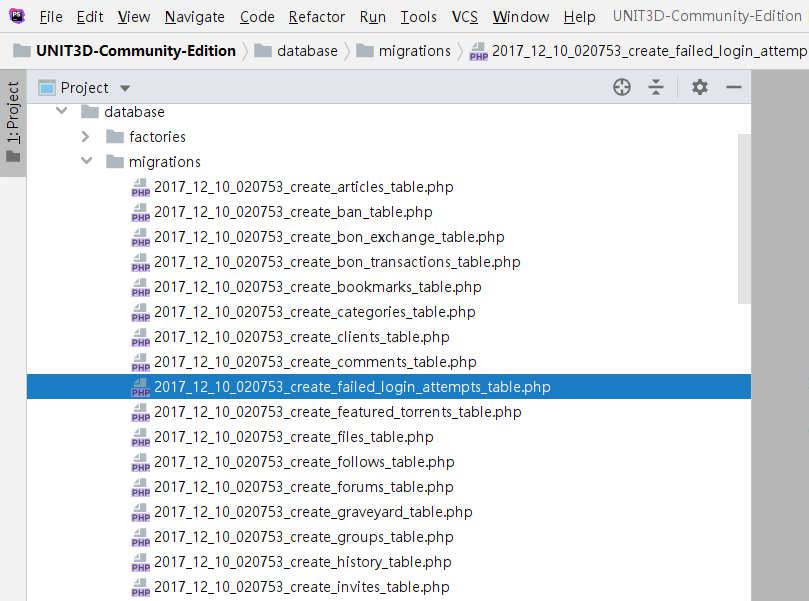
\includegraphics[width=\textwidth]{support-files/3.1-phpstorm-folder-structure-4.png}
		\caption{ }
		\label{fig:torrent_in_bencode}
	\end{subfigure} \\
	% \makebox[0.05\textwidth]{}
    \begin{subfigure}{0.3\textwidth}
		\centering
		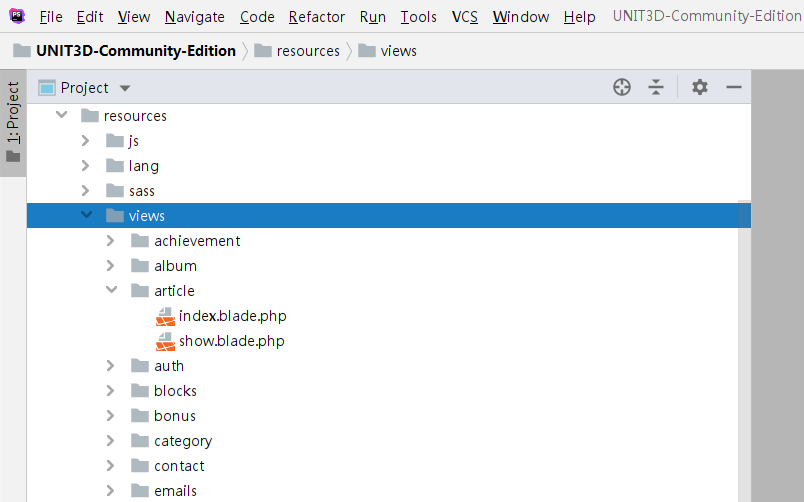
\includegraphics[width=\textwidth]{support-files/3.1-phpstorm-folder-structure-5.png}
		\caption{ }
		\label{fig:torrent_in_bencode}
	\end{subfigure}
	\makebox[0.05\textwidth]{}
    \begin{subfigure}{0.3\textwidth}
		\centering
		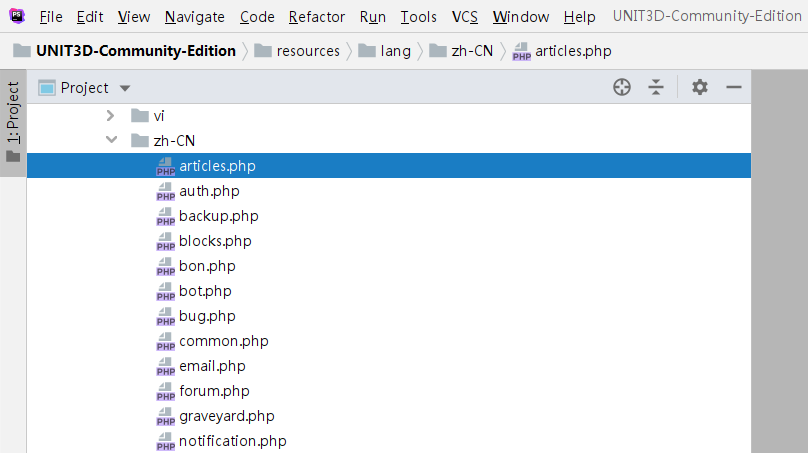
\includegraphics[width=\textwidth]{support-files/3.1-phpstorm-folder-structure-6.png}
		\caption{ }
		\label{fig:torrent_in_bencode}
	\end{subfigure} \\
	% \makebox[0.05\textwidth]{}
	\caption{在PhpStorm中看到的目录结构}
	\label{fig:phpstorm}
\end{figure}

\section{功能增删与调整}

\subsection{中文本地化}

未经修改的原始开源版本有开发者负责将英语的词汇进行机器翻译, 使之能够勉强本地化使用。然而作为母语是中文的用户, 机器翻译并不能满足笔者的要求。为此, 笔者修改了`/resources/views/, /resources/lang/'中的内容。

原版中已经有大量硬编码进视图的英语词汇。笔者的工作是将其一一剔除替换成可被取引用的形式。然后针对`/resources/lang/'中已有机器翻译的词汇, 进行一一校对、润色。


\subsection{数据表字段调整}

因为NexusPHP中有比较关键的字段, 如种子描述的副标题, 再UNIT3D中并没有对应的字段, 所以为了接下来的迁移工作, 必须要对UNIT3D的数据表进行字段的调整。

笔者主要的工作是在`/database/migrations/'目录中增加数据库改动迁移脚本, 同时要编写回溯的脚本, 以便于数据库的回滚操作。

\subsection{迁移NexusPHP数据表}

前期试运营的过程中使用了基于NexusPHP的天津大学北洋园TJUPT的开源版本\footnote{TJUPT项目页面: \url{https://github.com/sicalpath/tjupt}}并投入实际运营, 积累了大量有效的用户数据。然而NexusPHP和UNIT3D的原始数据表完全不兼容, 因此需要编写表级别的迁移脚本进行迁移工作。

UNIT3D的代码贡献者中有编写好的迁移脚本模板, 与笔者一同参与开发的同好之一, robinWongM同学对从NexusPHP迁移数据库至UNIT3D具有不可替代的贡献同学的工作是将该脚本进行一定的修改, 以适配TJUPT的一些特定字段。笔者则审核该脚本, 进行必要的修改, 增加前述的副标题字段, 然后交付上线试运行。

\subsection{标签调整}
\label{subsec:tagadjust}

因为原始的标签系统有很多元信息被设为必要字段, 而NexusPHP中的标签系统相对不那么严谨, 只在发布种子的时要求发布者填写必要的信息的时候根据输入的内容在种子标题字段中按照``[XX]''的形式用方括号括起相应的标签。 

然而UNIT3D独立实现了一个基于元信息联网查询的标签功能, 通过解析种子文件以及发布者输入的种子文件内容元信息, 解析出相应的字段, 如电影标题、电影对应的IMDB\footnote{IMDB: 一个互联网电影数据库, \url{https://www.imdb.com/}} ID等, 然后根据标题和ID向IMDB的API发起查询请求, 根据返回的结果里面的标签字段给发布到UNIT3D的种子打上标签, 继而录入数据库。

其中IMDB在国内的连接性并不理想, 导致在接下来刚开始开发测试的过程中, 不断出现500错误。为此, 笔者需要进行标签功能的剔除, 以避免这类因为网络连接性原因导致的极为影响用户体验的错误发生。

\subsection{实现投票功能}

在初期开发测试的过程中, 因为NexusPHP有简单但使用的投票功能, 初看UNIT3D UI的时候也发现了其投票功能。然而实际测试后发现, 该功能是只留了UI元素的桩功能, 并没有对接到数据库的持久化实现。加上投票页面有不少前端范畴的小错误, 需要一并修改。

\subsection{实现鉴权日志记录功能}
\label{subsec:auth}

由于PT网站的私密性质, 导致通常而言其用户会员制度会受到不怀好意的使用者的挑战。一般来说, PT网站为了促进种子的可持续分享, 会以用户的上传/下载量为指标评估这个用户对网站的贡献。上传/下载量完全根据BT客户端向Tracker发起HTTP GET请求所带的参数这一单一途径取得, 因此, 很容易通过伪造请求, 或是拦截、修改HTTP GET请求中的参数向Tracker谎报虚假的上传/下载量。

为了防止作弊的产生, 诸如NexusPHP等较早写就的PT系统会带有完善的Auth-Logging(鉴权行为日志记录)功能, 即将每一次带鉴权的操作, 比如上述这一通过Passkey (用户密钥, 包含在GET请求参数中, 作为BT客户端在无法使用Cookie进行HTTP通信交互情况下的用户鉴权标识符)向Tracker汇报(Announce)流量的操作, NexusPHP会将这次GET请求的源IP, 请求时间, 汇报的上传/下载流量长度, BT客户端的`User-Agent'标识符记录到数据库的日志表中, 以便将来对日志进行数据筛查、挖掘等处理的时候查明其中的作弊行为。

UNIT3D因为原作者设计理念的不同, 不具有该功能。作者的一个信念是: 如果你要作弊, 那就应该高明到不被服务器发现, 比如透过虚拟专用网络(VPN), 伪造用户身份信息等更加高超的手段, 而不是简单修改HTTP请求里的参数, 否则这样的作弊就是愚蠢的行为。而且不得不提的是, 由于每个用户都可能正在分享大量的种子, 鉴权行为日志记录带来的性能开销无法被简单忽略。因此, 作者并未开发该功能。

然而国内用户的使用状况不允许笔者及同好们运营的系统有这样的严重隐患。通过与原作者的沟通\footnote{见Github Issue: \url{https://github.com/HDInnovations/UNIT3D-Community-Edition/issues/1151}}, 笔者一方决定单独实现一个可选的鉴权日志记录功能。只有在开关打开的情况下, 才会向日志表中记录每次带鉴权的操作。这样既满足部分如笔者一方的网站运营方的严苛需求, 又不为不需要这一功能的PT服务端程序使用者带来不必要的性能开销。





